Para aliar a teoria com a prática, vamos 
começar desenvolvendo um novo projeto de 
back-end Java Web no Eclipse. Os projetos desenvolvidos no CPD/UnB 
na linguagem Java são do tipo Maven Project.

\section{Usando o Wizard New Maven Project}

Vá no menu File/New da IDE Eclipse e clique na opção 
Maven Project. Se a opção Maven Project não aparecer, localize-a dentro da opção Other.

\begin{figure}[htb]
\centering
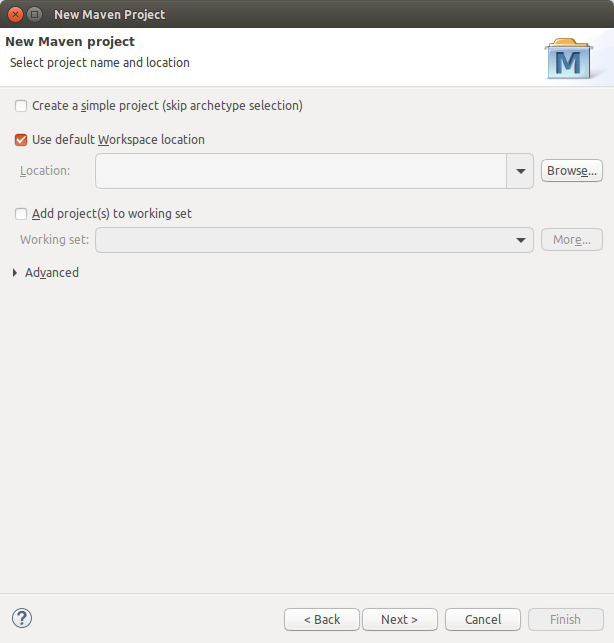
\includegraphics[scale=0.4]{/img/NewMavenProject_01.png}
\caption{New Maven Project Wizard - Seleção local projeto.}
\label{fig_new_maven_project_01}
\end{figure}
\FloatBarrier

A tela que se abre (Figura \ref{fig_new_maven_project_01}) 
é um Wizard para para a criação de um projeto Maven, que é o tipo de projeto
Java EE que usamos no CPD/UnB. Nesta primeira etapa, deve-se escolher 
o local onde será armazenado o código fonte do projeto que por padrão
é a workspace (marque a opção Use default Workspace location).

Na próxima tela, selecione o archetype da nova arquitetura para gerar
um projeto com o esqueleto padrão da arquitetura Erlangms. Para isso, 
selecione o item archetype unb-modulo-erlangms-archetype da lista, 
conforme ilustra a Figura \ref{fig_new_maven_project_02}.

\begin{figure}[htb]
\centering
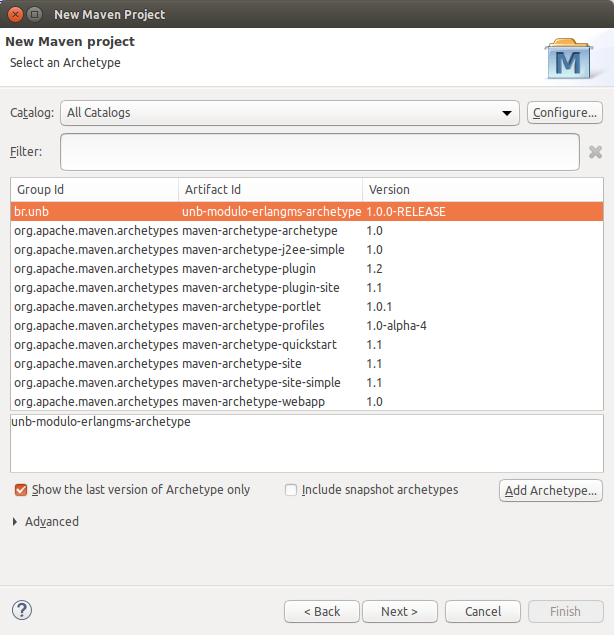
\includegraphics[scale=0.6]{/img/NewMavenProject_02.png}
\caption{New Maven Project Wizard - Seleção archetype.}
\label{fig_new_maven_project_02}
\end{figure}
\FloatBarrier

A partir de agora, devemos informar algumas informações importantes 
para o \textit{New Maven Project} criar nossa aplicação Java Web:

\begin{enumerate}[(a)]
   \item{GroupId} -- namespace base do projeto;
   \item{Artifact Id} -- nome do projeto;
   \item{Version} -- versão do pacote do projeto;
   \item{Package} -- namespace completo do package.
\end{enumerate}
  
Assim, no campo GroupId informe br.unb; 
no campo Artifact Id informe o nome do seu projeto (por exemplo, unb\_aula neste guia);
no campo Version informe a versão do projeto. O último
campo (Package) é gerado automaticamente pela IDE. A Figura \ref{fig_new_maven_project_03}
ilustra esta etapa do processo de criação da aplicação.

\begin{figure}[htb]
\centering
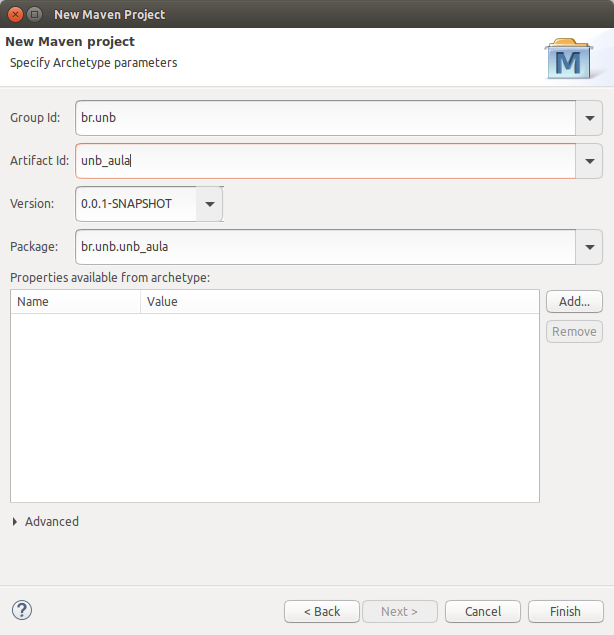
\includegraphics[scale=0.7]{/img/NewMavenProject_03.png}
\caption{New Maven Project Wizard - Informações sobre o projeto.}
\label{fig_new_maven_project_03}
\end{figure}

Pronto, podemos clicar em Finish para criar o projeto. A Figura \ref{fig_estrutura_proj} 
ilustra o painel Project Explorer com a estrutura do projeto na arquitetura Erlangms.


\begin{figure}[htb]
\centering
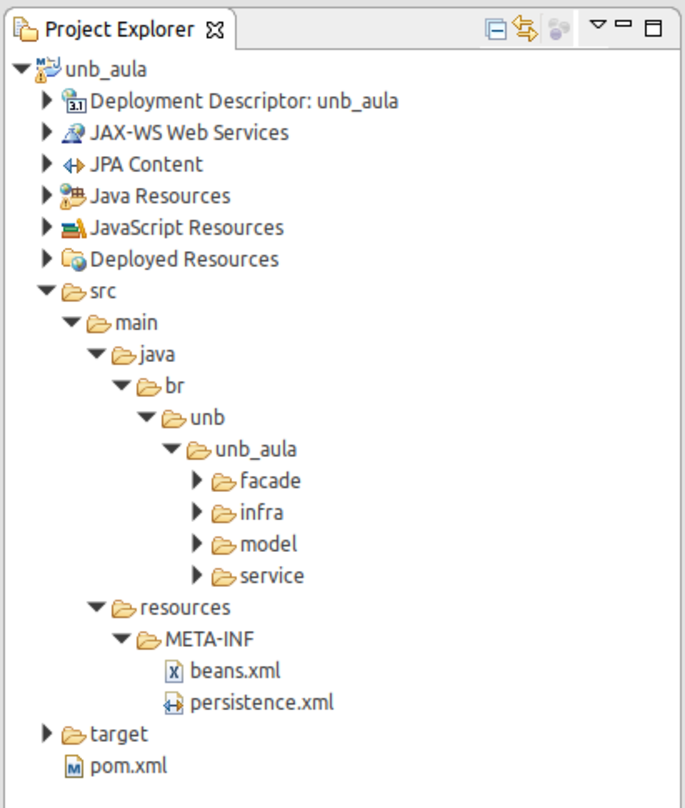
\includegraphics[scale=0.83]{/img/EstruturaProj.pdf}
\caption{Estrutura do Novo Projeto na arquitetura Erlangms.}
\label{fig_estrutura_proj}
\end{figure}
\FloatBarrier




\section{Dependências do Projeto}

Em um projeto Java Web do tipo Maven, existe um arquivo especial chamado \textit{pom.xml} onde
são informadas as dependências do projeto. As dependências geralmente são bibliotecas 
ou frameworks que oferecem algo útil para as aplicações. O Código \ref{fig:dependencias_proj}
exibe as dependências do projeto.


\lstset{
        basicstyle=\footnotesize,
        numbers=left,
        numberstyle=\footnotesize,
        tabsize=2,
        numbers=none,
        rulesepcolor=\color{blue}}
\renewcommand{\lstlistingname}{Código}             
\begin{lstlisting}[caption=Dependências na nova arquitetura., label=fig:dependencias_proj] 
<dependencies>
		<dependency>
			<groupId>br.erlangms</groupId>
			<artifactId>ems_java</artifactId>
			<version>1.0.0</version>
		</dependency>

		<dependency>
			<groupId>javax</groupId>
			<artifactId>javaee-api</artifactId>
			<version>7.0</version>
			<scope>provided</scope>
		</dependency>

		<dependency>
			<groupId>org.hibernate</groupId>
			<artifactId>hibernate-entitymanager</artifactId>
			<version>4.3.11.Final</version>
			<scope>provided</scope>
		</dependency>
</dependencies>
\end{lstlisting}

A seguir, uma breve descrição sobre o objetivo de cada dependência:
	
\begin{itemize}

\item{\bf ems\_java} é o SDK Java do Erlangms para comunicação com o barramento ems-bus. 
Contém um conjunto mínimo de classes para construir Web-services agnósticos, ou seja, 
de forma mais neutra possível. O código fonte do SDK está 
disponível em \url{https://github.com/erlangMS/sdk}.

\item{\bf Java EE 7} é a base na qual as aplicações Java Edição Enterprise são construídas. 
Convém salientar que na arquitetura anterior (Fast), a versão utilizada é a 6. 

\item{\bf hibernate-entitymanager} é o framework de persistência utilizado para a camada
de persitência. 

\end{itemize}



\section{Persistência do Projeto}

Outro importante arquivo em um projeto Java Web é o 
persistence.xml onde está configurado o banco de dados
que será utilizado. Inicialmente, 
este arquivo está configurado para utilizar
um banco de dados em memória. 

Assim, pode-se desenvolver o back-end e
até mesmo fazer deployment no JBoss/Wildfly pois as tabelas são automaticamente geradas de acordo 
com os modelos (ou POJOs) encontrados no projeto.

O Código \ref{fig:persistence_proj} exibe a configuração de persistência do projeto.


\lstset{
        basicstyle=\footnotesize,
        numbers=left,
        numberstyle=\footnotesize,
        tabsize=1,
        numbers=none,
        rulesepcolor=\color{blue}}
\renewcommand{\lstlistingname}{Código}             
\begin{lstlisting}[caption=Arquivo persistence.xml., label=fig:persistence_proj] 
<?xml version="1.0" encoding="UTF-8" ?>
<persistence xmlns:xsi="http://www.w3.org/2001/XMLSchema-instance"
  xsi:schemaLocation="http://java.sun.com/xml/ns/persistence http://java.sun.com/xml/ns/persistence/persistence_2_0.xsd"
  version="2.0" xmlns="http://java.sun.com/xml/ns/persistence">
  <persistence-unit name="service_context" transaction-type="JTA">
	<provider>org.hibernate.ejb.HibernatePersistence</provider>	
    <properties>
      <property name="javax.persistence.jdbc.driver" value="org.apache.derby.jdbc.EmbeddedDriver" />
      <property name="javax.persistence.jdbc.url" value="jdbc:derby://localhost:1527/database;create=true" />
      <property name="javax.persistence.jdbc.user" value="test" />
      <property name="javax.persistence.jdbc.password" value="test" />

	  <!-- <property name="jboss.entity.manager.factory.jndi.name" value="java:/service_context" /> -->
	  <property name="hibernate.show_sql" value="true" />	
  	  <property name="hibernate.format_sql" value="false"/>
  	  <property name="hibernate.jdbc.use_scrollable_resultset" value="false"/>	
  	  <property name="hibernate.hbm2ddl.auto" value="create" /> 
    </properties>
  </persistence-unit>
</persistence>
\end{lstlisting}

